\def\VCDate{2016/04/15}\def\VCVersion{(Current)}
\documentclass{article}
\usepackage{ProofPower,verbatim,graphicx,float}
\usepackage{amsmath,amsfonts,fpic,color,pstricks,xcolor,pstricks-add}
\usepackage{underscore,listings,hyperref}
\usepackage[margin=0.5in,paperwidth=6in,paperheight=5in]{geometry}
\title{gcd function in sml, C, and asm}
\setcounter{secnumdepth}{0}
\begin{document} 
\author{Saw Thinkar Nay Htoo}
\maketitle

\clearpage

\hypertarget{p2}{\section{gcd}}

The greatest common divisor (gcd) of two positive natural numbers is the largest natural 
number that exactly divides both numbers. 
The gcd of 14 and 12 is 2, while the gcd of 14 and 11 is 1.
The gcd is given by this specification:
\[ \text{gcd} : (\mathbb{N} \times \mathbb{N}) \rightarrow \mathbb{N} \]
\[ \text{gcd}(m,n) = \text{max}\{d \in \mathbb{N} \vert m \bmod d = 0 \land n \bmod d = 0\} \]

One {\it algorithm} for calculating the gcd follows Euclid's method. If, for two positive natural
numbers $m$ and $n$, we have that $m>n$, then the gcd of $m$ and $n$ is defined by:
\[ \text{euclid} : (\mathbb{N} \times \mathbb{N}) \rightarrow \mathbb{N} \]
\[ \text{euclid}(m,n) = 
     \left\{
        \begin{array}{lr}
             \text{euclid}(n,m \bmod n), & \text{if} \; n > 0 \\
             m, & \text{otherwise}
        \end{array}
      \right.
 \]
\clearpage

\hypertarget{p3}{\section{gcd in sml}}
This can be written in SML like this:
\begin{GFT}{SML}
\+fun euclid m n = if n > 0\\
\+                    then euclid n (m mod n)\\
\+                    else m ;\\
\+euclid 558 198;  (* expect 18 *)\\
\end{GFT}

Although a short program, we may not be familiar with the use of recursion because it is not commonly used for C programs due to its inefficiency. But let's implement it that way anyway to follow the math definition more closely.\\
\section{SML code result}
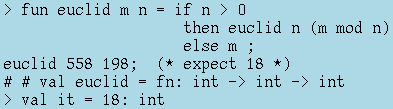
\includegraphics[scale=0.6]{euclidsml.png}
\clearpage

\hypertarget{p4}{\section{gcd in c}}
\begin{GFT}{C source code written to file lab3.c}
\+\#include <stdio.h>\\
\+int euclid(int m, int n)\\
\+\{\\
\+  if( n > 0) return euclid(n, m \% n);\\
\+  else return m;\\
\+\}\\
\+int main()\\
\+\{\\
\+  printf("GCD output = \%i\Backslash{}n",euclid(558,198));\\
\+  return 0;\\
\+\}\\
\end{GFT}
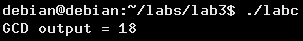
\includegraphics[scale=0.5]{euclidc.png}
\clearpage
The first line of this C code is an include to get access to the library. We need it here to use printf.
\lstinputlisting[language=C,linerange={1-1}]{lab.c}
In ASM, we do not need to include any files in order to link to the C library, so we can skip this.
\subsection{gcd in c: euclid function}
\lstinputlisting[language=C,linerange={2-6}]{lab.c}
These lines are the function definition. There are several techniques to be studied to implement it in assembler:
\begin{itemize}

\item syntax for function definitions\\
C: \\
\verb|int euclid(){}|\\
ASM: function is declared using "euclid:"\\
\verb|euclid:|\\

\item parameter passing \\
C: \\
\verb|int m, int n|\\
ASM: variables are placed in stack.\\
\verb|push $198|\\
\verb|push $558|\\

\item decision (if statement)\\
C: \\
\verb|if() return euclid();|
\verb|else return m;|
ASM: the procedure will simply jump to endif.\\
\verb|jmp endif|\\
\verb|...|\\
\verb|endif:|\\

\item conditional (relational expression to compare values) \\
C:\\
\verb|if (n>0) return euclid()|\\
\verb|else reutrn m;|\\
\verb||\\
\clearpage
ASM:eax is compared with zero. If eax is equal to zero, it will go to "else". If not it willl keep repeating the first function.\\
\verb|cmp $0, %eax|\\
\verb|jle else|\\
\verb|...|\\
\verb|else:|\\
\verb|...|\\

\item return statement \\
C:\\
\verb|return|\\
ASM: "ret" is simply used as "return"\\
\verb|ret|\\

\item calling a function (recursively in this case) \\
C:\\
\verb|euclid(558,198)|\\
ASM: In ASM, function called using "call function-name"\\
\verb|call euclid|\\

\clearpage
\item calculating modulus \\
C: \\
\verb|m % n|\\
ASM: two numbers are kept in the stack for one operation then placed in ebx and eax registers. edx is set to zero to clear off the previous value. idiv command is used to divide eax by, ebx giving out the remainder of edx. \href{https://goo.gl/h2TVeq}{Click here} for detailed explanation for idiv.\\
\verb|mov 12(%ebp), %ebx|\\
\verb|mov  8(%ebp), %eax|\\
\verb|mov $0, %edx|\\
\verb|idiv %ebx|\\
\end{itemize}

\clearpage\subsection{gcd in asm: main}
%\lstinputlisting[language=C,linerange={7-11}]{lab.c}
The main function is simpler, but we need to also learn how to: 
\begin{itemize}
\item call printf
\item end the program
\end{itemize}
ASM code is put in the ``text'' section. The entry point is named ``_start''. It is a label (indicated by the colon). We make it global so the linker will make it visible to be called externally (by the operating system).
\begin{GFT}{ASM source code written to file lab3.s}
\+.text\\
\+.globl \_start\\
\+\_start:\\
\end{GFT}
\clearpage
printf needs 2 parameters: a format string and a value. That value must be determined by called our function euclid. Return values are found in the EAX register. The euclid function also requires 2 parameters which must be pushed onto the system stack so they can be retrieved within the function. Parameters are pushed right to left (the C convention). Immediate (literal) values are prefixed with the \$ sign. Register names are prefixed with the \% sign.
\begin{GFT}{ASM source code appended to file lab3.s}
\+push \$198\\
\+push \$558\\
\+call euclid\\
\+add \$8, \%esp \#two of them 4 bytes each\\
\+.data\\
\+fmt: .string "GCD output = \%d\Backslash{}n"\\
\+.text\\
\+push \%eax\\
\+push \$fmt\\
\+call printf\\
\+add \$8, \%esp\\
\end{GFT}
\clearpage
The program is ended by calling software interrupt 0x80. The 1 in EAX means exit command and the 0 in EBX is the convention to mean program had no errors.
\begin{GFT}{ASM source code appended to file lab3.s}
\+mov \$1,\%eax\\
\+mov \$0,\%ebx\\
\+int \$0x80\\
\end{GFT}
\clearpage\subsection{gcd in asm: euclid function}
The euclid function uses the same technique of creating a label to indicate start of function. It ends with the ret instruction. The first 2 instructions set up a stack frame base pointer (EBP) to give us access to paramters even if the stack pointer (ESP) moves.

\begin{GFT}{ASM source code appended to file lab3.s}
\+euclid:\\
\+push \%ebp\\
\+\\
\end{GFT}
Now we can access the 2 parameters using register EBP. 4 bytes above EBP is the return address, 8 is the 1st parm, and 12 is the second. i.e.
\begin{description}
\item[n] is on stack at \verb|12(%ebp)|
\item[m] is on stack at \verb| 8(%ebp)|
\end{description}
The if statement has to be simulated by branching to labels depending of results of doing the comparison of n to zero.
\begin{GFT}{ASM source code appended to file lab3.s}
\+mov \%esp,\%ebp\\
\+mov 12(\%ebp),\%eax\\
\+cmp \$0,\%eax\\
\+jle else\\
\end{GFT}
This is the ``then'' part of the if statement. We need to calculate $m \mod n$ and call euclid again!  Integer division is done by putting dividend in EDX:EAX as 64-bit value, and divisor in EBX. The remainder will be in EDX.
\begin{GFT}{ASM source code appended to file lab3.s}
\+mov 12(\%ebp), \%ebx\\
\+mov 8(\%ebp), \%eax\\
\+mov \$0, \%edx \# clear upper 32 bits of the 64-bit divident edx:eax\\
\+idiv \%ebx \# modulus is in edx (quotient is in eax)\\
\+push  \%edx\\
\+push \%ebx\\
\+call euclid\\
\+add \$8,\%esp\\
\+jmp endif\\
\+else:\\
\+mov 8(\%ebp),\%eax\\
\+endif: \\
\end{GFT}
\clearpage
These last 2 instructions undo the first 2--they restore the original stack as it was found on entry to the function.
\begin{GFT}{ASM source code appended to file lab3.s}
\+mov \%ebp,\%esp\\
\+pop \%ebp\\
\+ret \\
\end{GFT}
Here is output from running the ASM program:\\
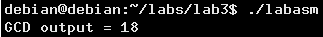
\includegraphics[scale=0.8]{asmfinal.png}
\clearpage




\section*{This is my own lab explanation.}
I made this lab report as simple as possible so that anyone without computing knowledge will be able to understand the content of this lab. In this lab, there are two most important things to understand fully: Euclidean Algorithm and Stackframe. \\

\section*{What is Euclidean Algorithm}
According to wikipedia, \href{https://goo.gl/H3t3BI}{Euclidean algorithm} is an efficient method for computing \href{https://goo.gl/iKdLpd}{the greatest common divisor(gcd)} of two numbers, the largest number that divides both of them without leaving a remainder. Below is the sample long division components compared with registers. Ok, what are those eax, ebx and edx? They are \href{https://goo.gl/2So2Hx}{general purpose registers}, where values are stored to do the calculation, and they have \href{https://goo.gl/Nrc0GJ}{specific purposes}. We will have to deal more with these registers when we write this algorithm using assembly language.\\
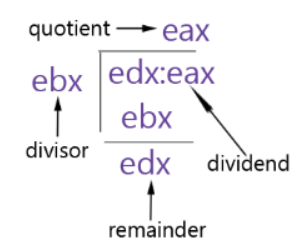
\includegraphics[scale=0.4]{gcdsample.PNG}
\clearpage

Lets say there are two numbers: 558 and 198. As we can see below, in the first step, dividend, 558 is divided by divisor, 198, resulting the remainder of 162. Then the remainder, 162 becomes the divisor in the second step, dividing the new dividend, 198 to give the new result of the remainder which is 36. The same procedure is repeated until the divisor becomes zero. So in this case, the GCD of 558 and 198 is 18. \\
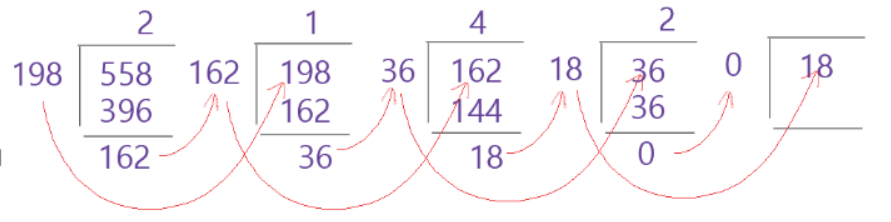
\includegraphics[scale=0.5]{gcd.PNG}\\
This \href{https://goo.gl/Lj5I2M}{link} is the youtube video explanation for Euclidean Algorithm.\\
Now if you feel confident enough with your Euclidean Algorithm understanding, try to answer GCD for these numbers: (255,245), (531,234) and (126,186).\\ 
Using this \href{https://goo.gl/neHGSK}{online GCD calculator} you can check your answer here.\\
\smallskip\\
\hyperlink{p2}{Click here} for the Euclidean Algorithm in mathematical expression.\\
\hyperlink{p3}{Click here} for the alogrithm written in \href{https://goo.gl/H5hWaQ}{SML functional programming language}.\\
\hyperlink{p4}{Click here} for the alogirthm written in \href{https://goo.gl/PqXN2H}{C programming language}.\\
\clearpage

\section*{Euclidean Algorithm in Assembly Language(ASM)}
Now, lets begin with what \href{https://goo.gl/4S1vKl}{assembly language} is. It is a low-level programming language. This programming language is simple to write codes, if you understand the concept well, but you will have to write a lot just for a short program of high-level programming languages such as C, C++, and so on. Below is the Euclidean Algorithm in ASM.\\
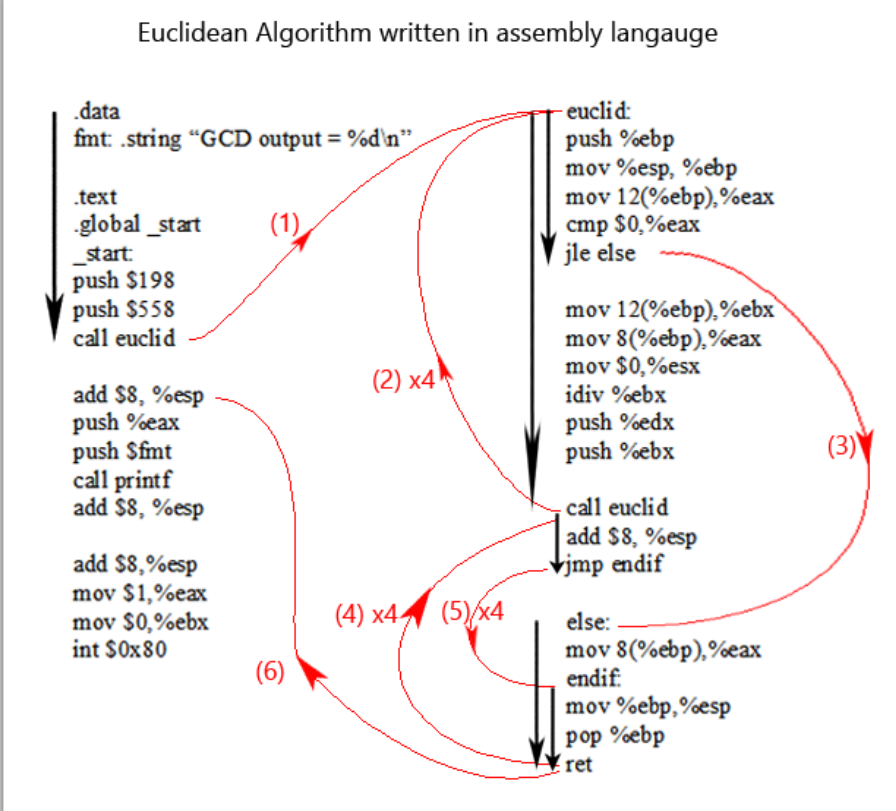
\includegraphics[scale=0.4]{euclidasm.PNG}
\clearpage

\section*{The Stackframe: 1}
\begin{minipage}{5cm}
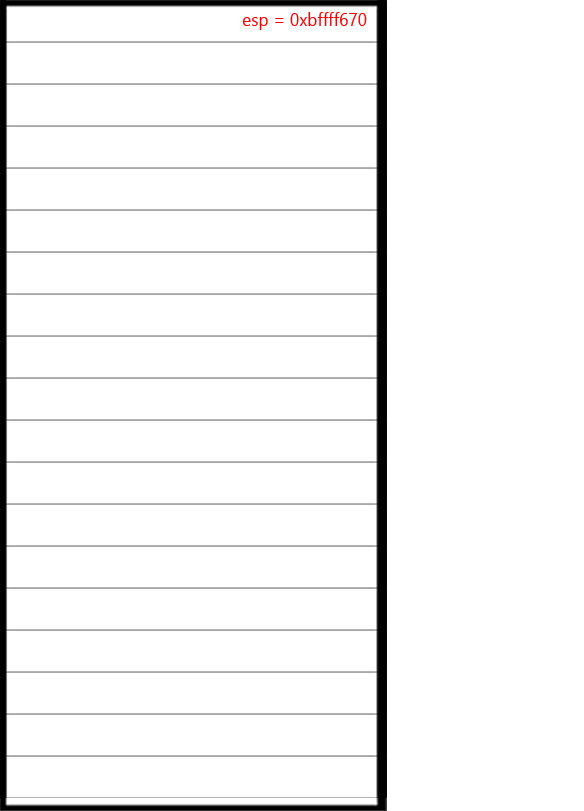
\includegraphics[scale=0.3]{s1.png}
\end{minipage}
\begin{minipage}{8cm}
This is the first time checking the stackframe before running the program.\\
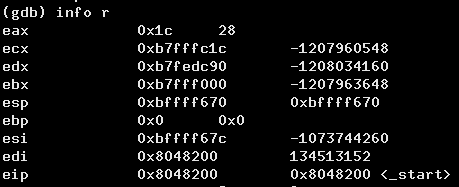
\includegraphics[scale=0.4]{info1.png} \\
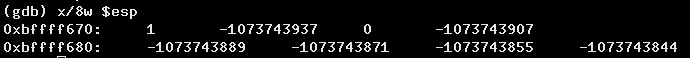
\includegraphics[scale=0.3]{x1.png} \\
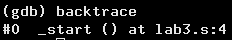
\includegraphics[scale=0.5]{bt1.png} \\
\end{minipage}
\clearpage

\section*{2}
\begin{minipage}{5cm}
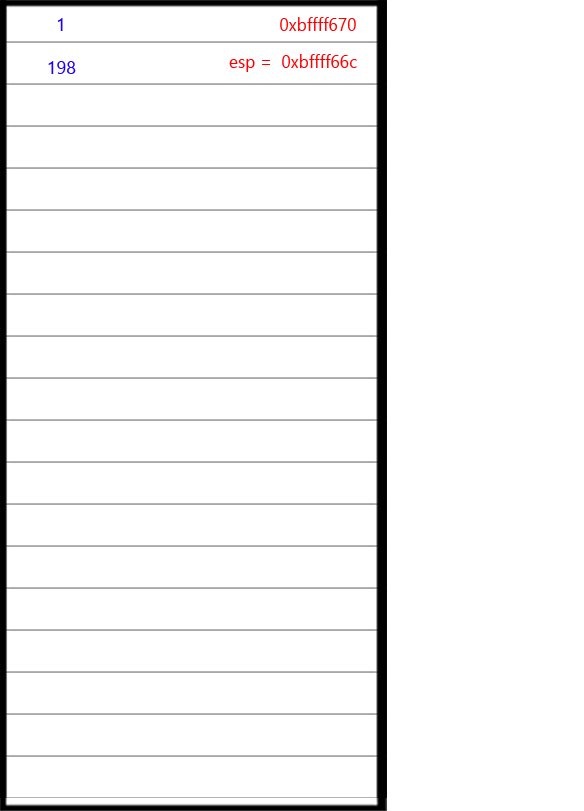
\includegraphics[scale=0.3]{s2.png}
\end{minipage}
\begin{minipage}{8cm}
\verb|push $198|\\
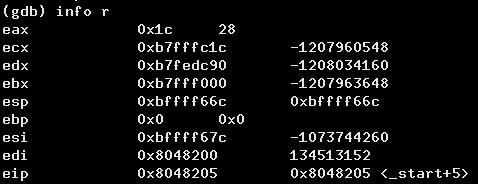
\includegraphics[scale=0.4]{info2.png} \\
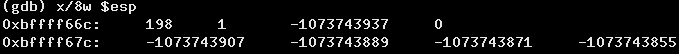
\includegraphics[scale=0.3]{x2.png} \\
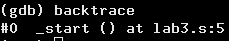
\includegraphics[scale=0.5]{bt2.png} \\
\end{minipage}
\clearpage

\section*{3}
\begin{minipage}{5cm}
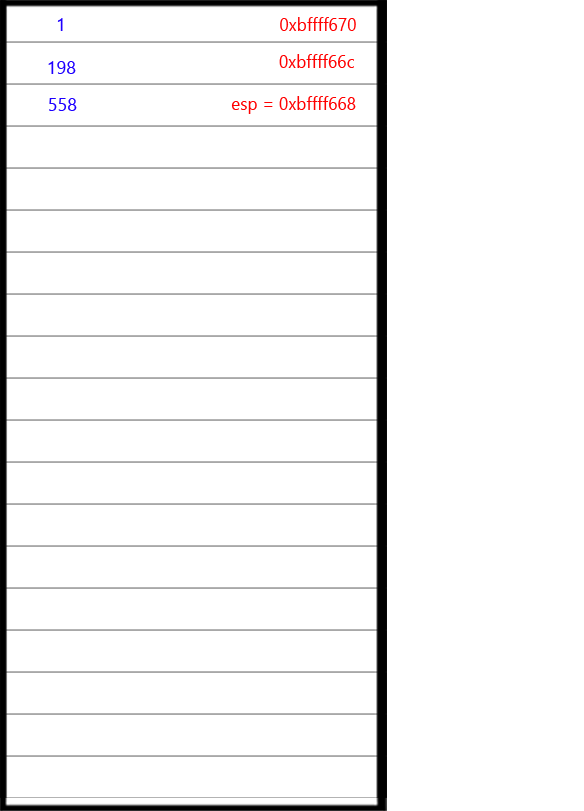
\includegraphics[scale=0.3]{s3.png}
\end{minipage}
\begin{minipage}{8cm}
\verb|push $558|\\
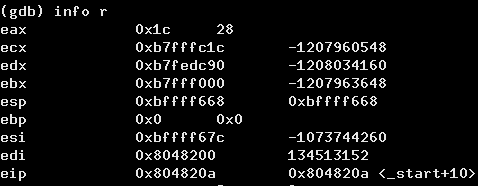
\includegraphics[scale=0.4]{info3.png} \\
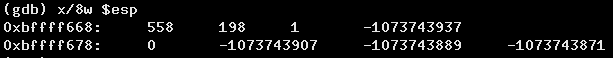
\includegraphics[scale=0.3]{x3.png} \\
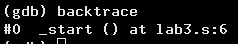
\includegraphics[scale=0.5]{bt3.png} \\
\end{minipage}
\clearpage

\section*{4}
\begin{minipage}{5cm}
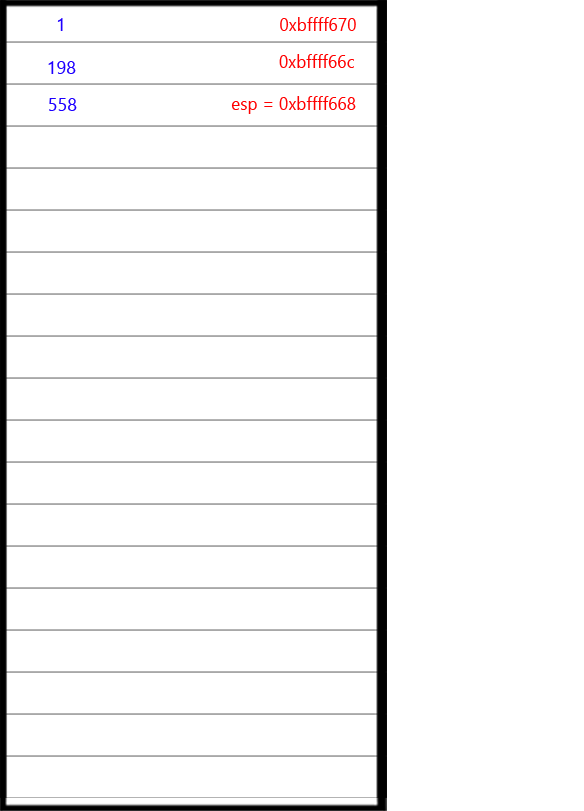
\includegraphics[scale=0.3]{s3.png}
\end{minipage}
\begin{minipage}{8cm}
\verb|call euclid|\\
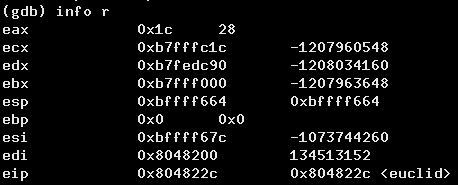
\includegraphics[scale=0.4]{info4.png} \\
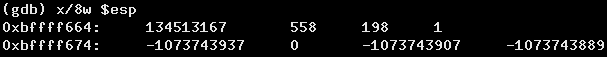
\includegraphics[scale=0.3]{x4.png} \\
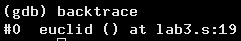
\includegraphics[scale=0.5]{bt4.png} \\
\end{minipage}
\clearpage

\section*{5}
\begin{minipage}{5cm}
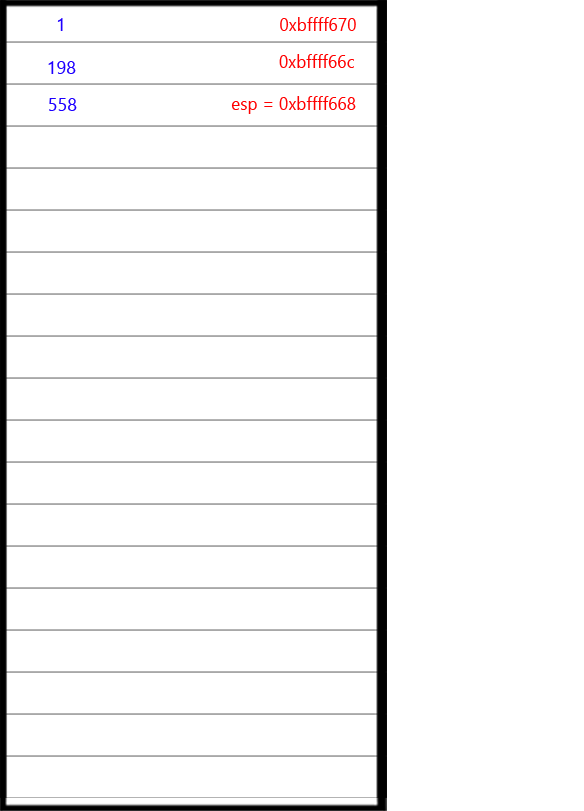
\includegraphics[scale=0.3]{s3.png}
\end{minipage}
\begin{minipage}{8cm}
\verb|push %ebp|\\
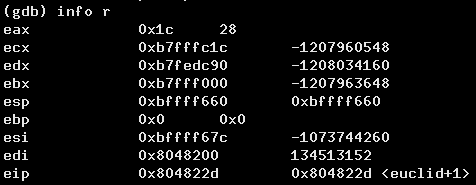
\includegraphics[scale=0.4]{info5.png} \\
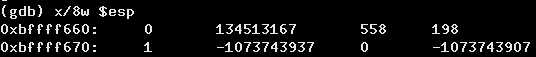
\includegraphics[scale=0.3]{x5.png} \\
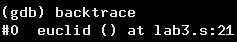
\includegraphics[scale=0.5]{bt5.png} \\
\end{minipage}
\clearpage

\section*{6}
\begin{minipage}{5cm}
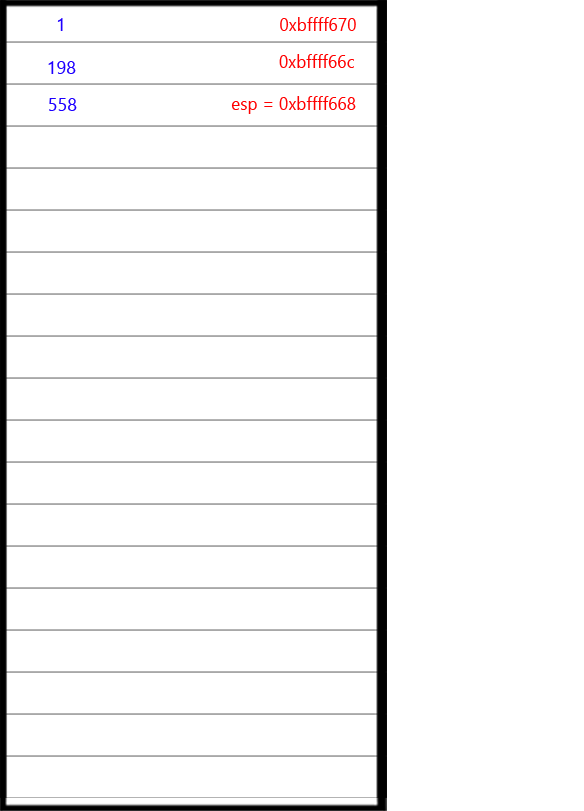
\includegraphics[scale=0.3]{s3.png}
\end{minipage}
\begin{minipage}{8cm}
\verb|mov %esp,%ebp|\\
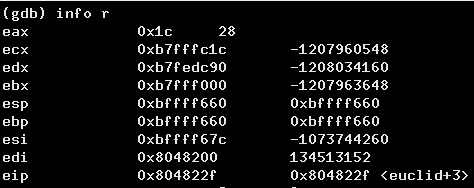
\includegraphics[scale=0.4]{info6.png} \\
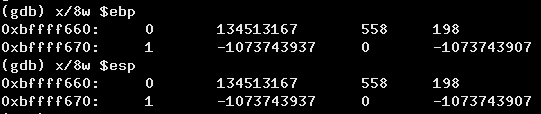
\includegraphics[scale=0.4]{x6.png} \\
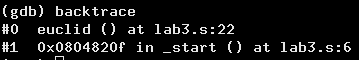
\includegraphics[scale=0.5]{bt6.png} \\
\end{minipage}
\clearpage

\section*{7}
\begin{minipage}{5cm}
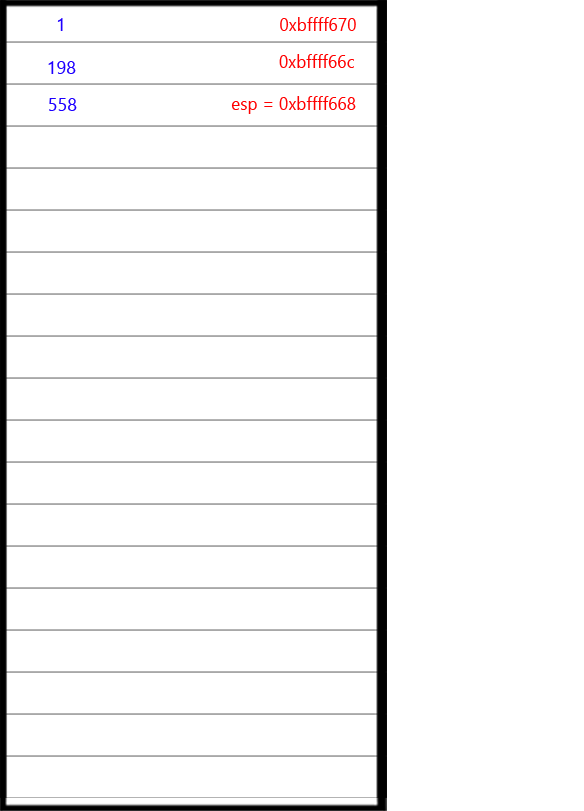
\includegraphics[scale=0.3]{s3.png}
\end{minipage}
\begin{minipage}{8cm}
\verb|mov 12(%ebp),%eax|\\
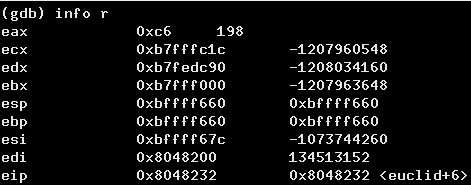
\includegraphics[scale=0.4]{info7.png} \\
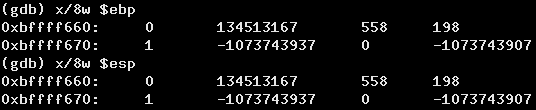
\includegraphics[scale=0.4]{x7.png} \\
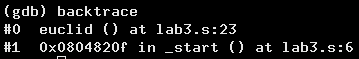
\includegraphics[scale=0.5]{bt7.png} \\
\end{minipage}
\clearpage

\section*{8}
\begin{minipage}{5cm}
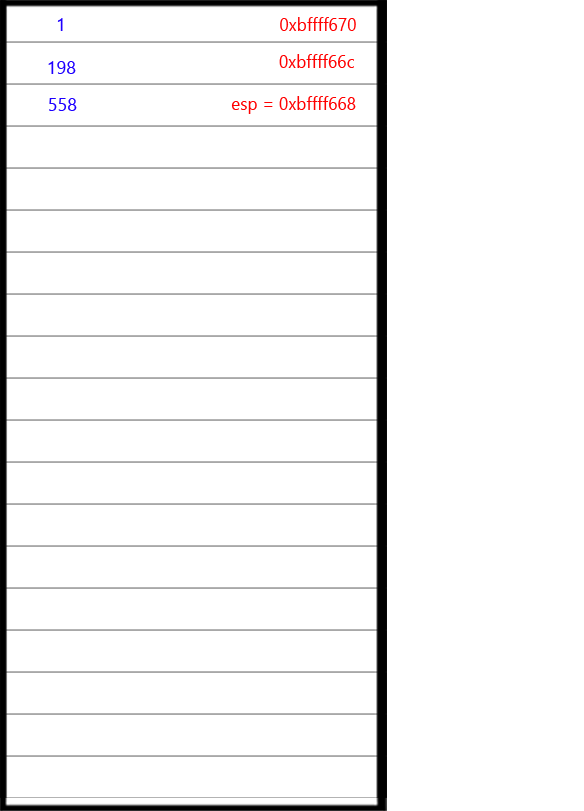
\includegraphics[scale=0.3]{s3.png}
\end{minipage}
\begin{minipage}{8cm}
\verb|cmp $0,%eax|\\
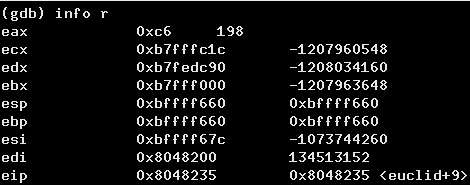
\includegraphics[scale=0.4]{info8.png} \\
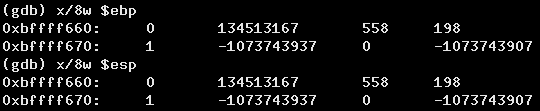
\includegraphics[scale=0.4]{x8.png} \\
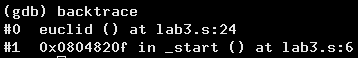
\includegraphics[scale=0.5]{bt8.png} \\
\end{minipage}
\clearpage

\section*{9}
\begin{minipage}{5cm}
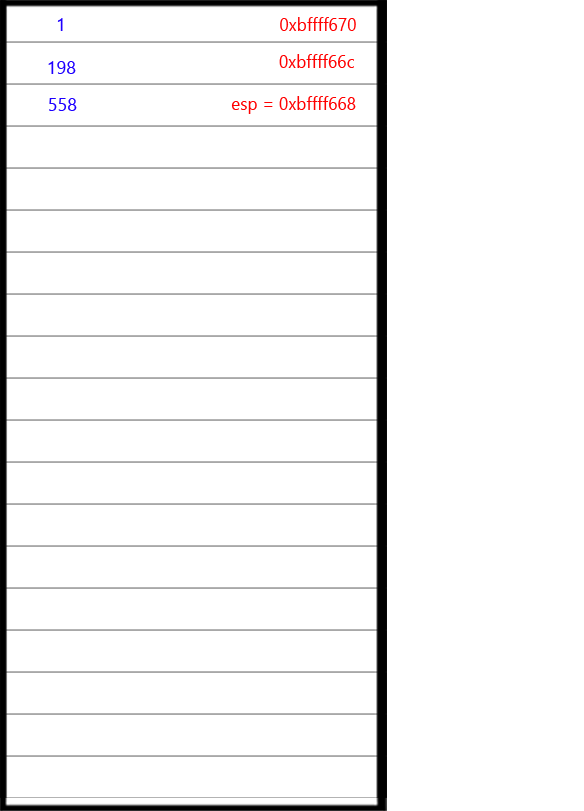
\includegraphics[scale=0.3]{s3.png}
\end{minipage}
\begin{minipage}{8cm}
\verb|jle else|\\
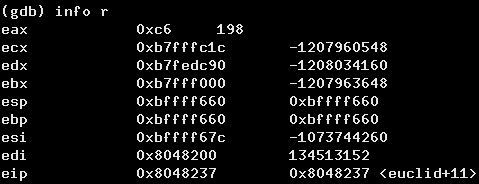
\includegraphics[scale=0.4]{info9.png} \\
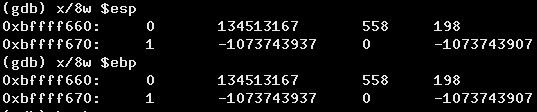
\includegraphics[scale=0.4]{x9.png} \\
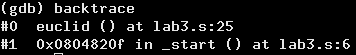
\includegraphics[scale=0.5]{bt9.png} \\
\end{minipage}
\clearpage

\section*{10}
\begin{minipage}{5cm}
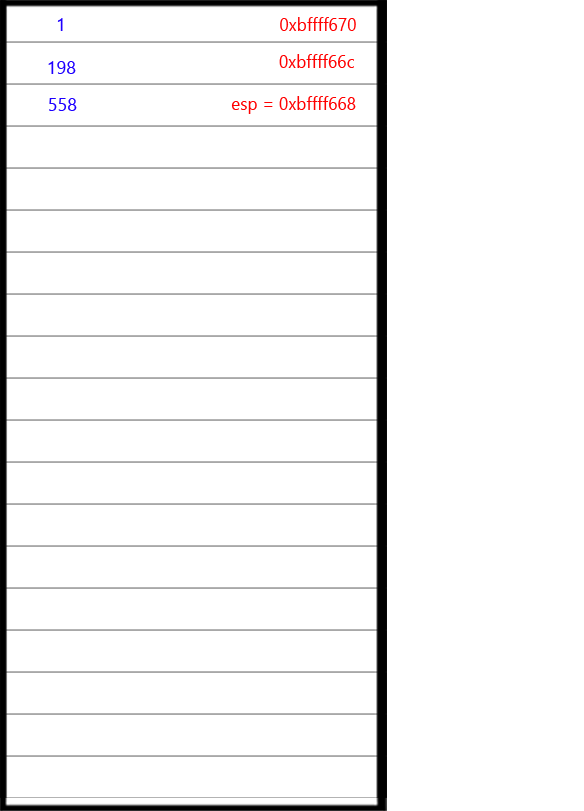
\includegraphics[scale=0.3]{s3.png}
\end{minipage}
\begin{minipage}{8cm}
\verb|mov 12(%ebp), %ebx|\\
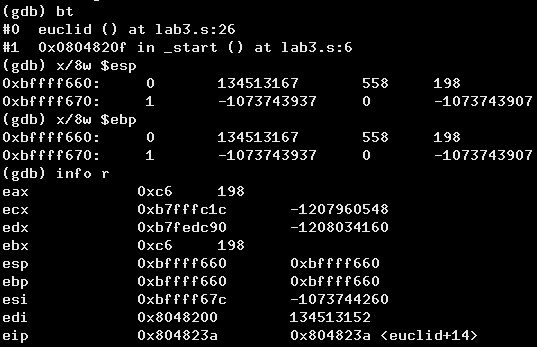
\includegraphics[scale=0.4]{bxi10.png} \\
\end{minipage}
\clearpage

\section*{11}
\begin{minipage}{5cm}
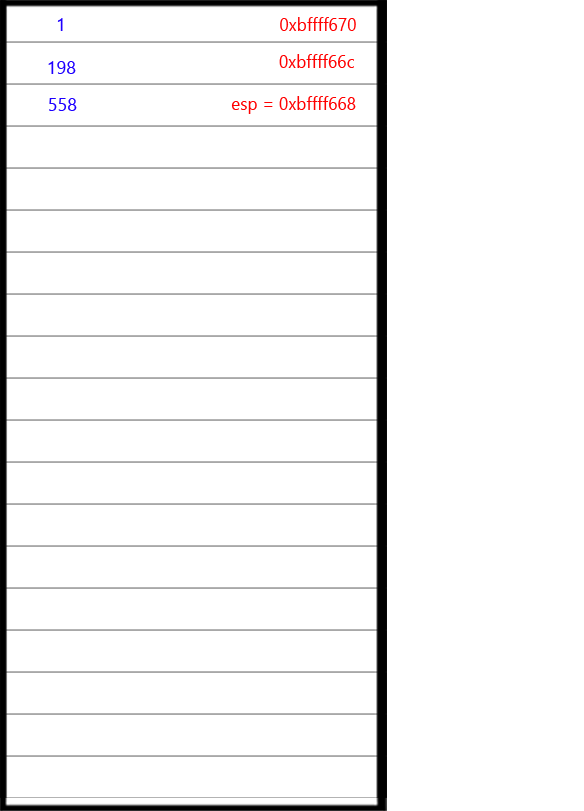
\includegraphics[scale=0.3]{s3.png}
\end{minipage}
\begin{minipage}{8cm}
\verb|mov 8(%ebp), %eax|\\
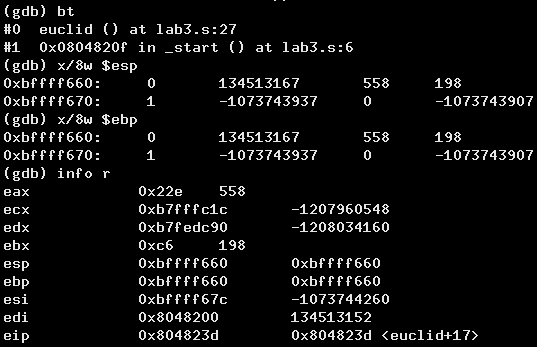
\includegraphics[scale=0.4]{bxi11.png} \\
\end{minipage}
\clearpage

\section*{121}
\begin{minipage}{5cm}
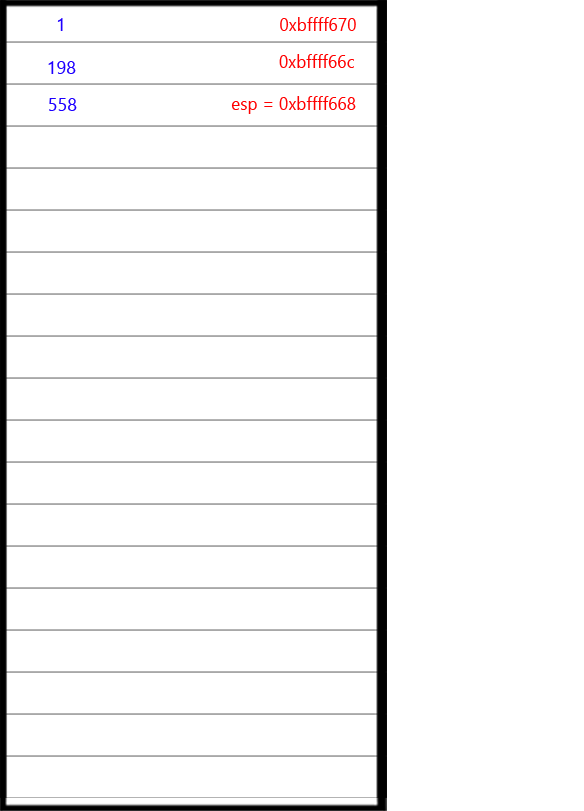
\includegraphics[scale=0.3]{s3.png}
\end{minipage}
\begin{minipage}{8cm}
\verb|mov 0, %edx|\\
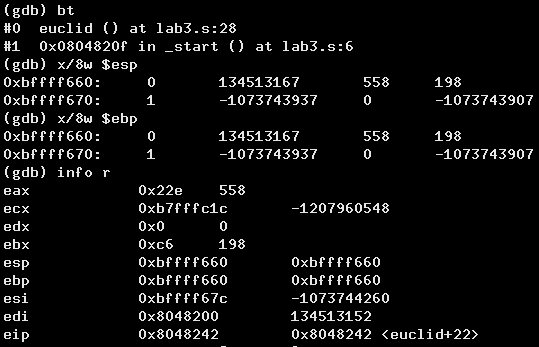
\includegraphics[scale=0.4]{bxi12.png} \\
\end{minipage}
\clearpage

\section*{13}
\begin{minipage}{5cm}
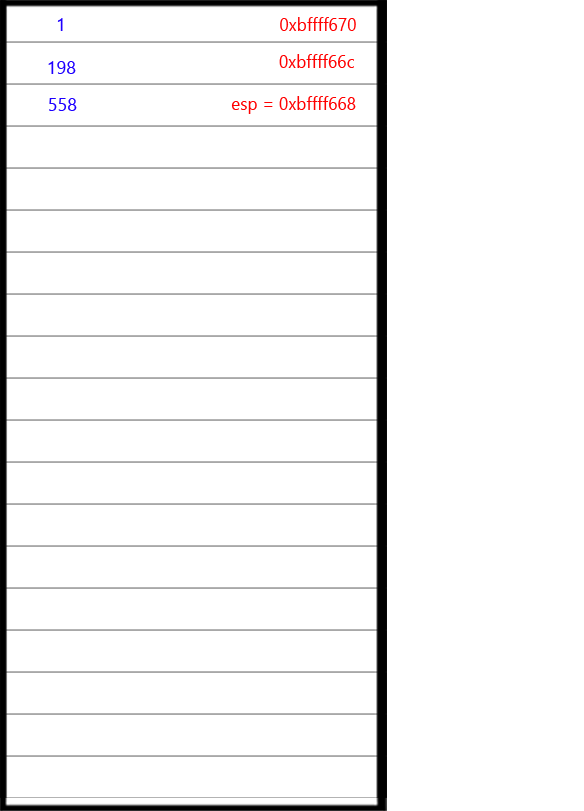
\includegraphics[scale=0.3]{s3.png}
\end{minipage}
\begin{minipage}{8cm}
\verb|idiv %ebx|\\
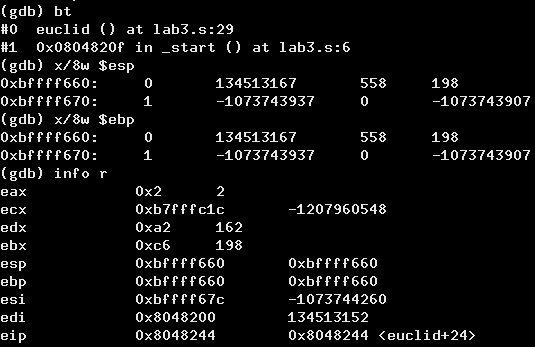
\includegraphics[scale=0.4]{bxi13.png} \\
\end{minipage}
\clearpage

\section*{14}
\begin{minipage}{5cm}
\includegraphics[scale=0.3]{s3.png}
\end{minipage}
\begin{minipage}{8cm}
\verb|push %edx|\\
\includegraphics[scale=0.4]{bxi14.png} \\
\end{minipage}
\clearpage

\section*{11}
\begin{minipage}{5cm}
\includegraphics[scale=0.3]{s3.png}
\end{minipage}
\begin{minipage}{8cm}
\verb|push %ebx|\\
\includegraphics[scale=0.4]{bxi15.png} \\
\end{minipage}
\clearpage

\section*{16}
\begin{minipage}{5cm}
\includegraphics[scale=0.3]{s3.png}
\end{minipage}
\begin{minipage}{8cm}
\verb|call euclid|
There are a few things happened aftering calling the euclid function, and they are not obviously seen in the gdb. But by seeing the address changes we can say what happened there.\\
\includegraphics[scale=0.4]{bxi16.png} \\
\end{minipage}
\clearpage

\section*{17}
\begin{minipage}{5cm}
\includegraphics[scale=0.3]{s3.png}
\end{minipage}
\begin{minipage}{8cm}
\verb|mov 12(%ebp), %eax|\\
\includegraphics[scale=0.4]{bxi17.png} \\
\end{minipage}
\clearpage

\section*{18}
\begin{minipage}{5cm}
\includegraphics[scale=0.3]{s3.png}
\end{minipage}
\begin{minipage}{8cm}
\verb|cmp $0,%eax|\\
\includegraphics[scale=0.4]{bxi18.png} \\
\end{minipage}
\clearpage

\section*{19}
\begin{minipage}{5cm}
\includegraphics[scale=0.3]{s3.png}
\end{minipage}
\begin{minipage}{8cm}
\verb|jle else|\\
\includegraphics[scale=0.4]{bxi19.png} \\
\end{minipage}
\clearpage

\section*{20}
\begin{minipage}{5cm}
\includegraphics[scale=0.3]{s3.png}
\end{minipage}
\begin{minipage}{8cm}
\verb|mov 12(%ebp), %ebx|\\
\includegraphics[scale=0.4]{bxi20.png} \\
\end{minipage}
\clearpage

\section*{21}
\begin{minipage}{5cm}
\includegraphics[scale=0.3]{s3.png}
\end{minipage}
\begin{minipage}{8cm}
\verb|mov 8(%ebp), %eax|\\
\includegraphics[scale=0.4]{bxi21.png} \\
\end{minipage}
\clearpage

\section*{22}
\begin{minipage}{5cm}
\includegraphics[scale=0.3]{s3.png}
\end{minipage}
\begin{minipage}{8cm}
\verb|mov $0, %edx|\\
\includegraphics[scale=0.4]{bxi22.png} \\
\end{minipage}
\clearpage

\section*{23}
\begin{minipage}{5cm}
\includegraphics[scale=0.3]{s3.png}
\end{minipage}
\begin{minipage}{8cm}
\verb|idiv %ebx|\\
\includegraphics[scale=0.4]{bxi23.png} \\
\end{minipage}
\clearpage

\section*{24}
\begin{minipage}{5cm}
\includegraphics[scale=0.3]{s3.png}
\end{minipage}
\begin{minipage}{8cm}
\verb|push %edx|\\
\includegraphics[scale=0.4]{bxi24.png} \\
\end{minipage}
\clearpage

\section*{25}
\begin{minipage}{5cm}
\includegraphics[scale=0.3]{s3.png}
\end{minipage}
\begin{minipage}{8cm}
\verb|push %ebx|\\
\includegraphics[scale=0.4]{bxi25.png} \\
\end{minipage}
\clearpage





\begin{GFT}{Text written to file labcode.sh}
\+docsml lab3.doc\\
\+as -gstabs -o lab.o lab3.s\\
\+ld -dynamic-linker /lib/ld-linux.so.2 -o labasm lab.o -lc -lX11\\
\+gcc -Wall -o labc lab3.c\\
\+\\
\end{GFT}
\begin{GFT}{Text written to file labcode2.sh}
\+gcc -Wall -o labc lab.c\\
\+gcc -Wall -o labasm lab.s\\
\+\\
\end{GFT}
\begin{GFT}{Text written to file labdoc.sh}
\+doctex lab3.doc\\
\+pptexenv /home/debian/texfot.pl pdflatex lab3.tex\\
\+\\
\end{GFT}
\begin{GFT}{Bourne Shell}
\+chmod 755 labcode2.sh\\
\+chmod 755 labcode.sh\\
\+chmod 755 labdoc.sh\\
\+\\
\end{GFT}
\end{document}
